% Chapter 6 reports the measured outcomes of the implemented methods.
% Content: handwritten-first reporting basis, LLM/VLM-based handwritten matrix,
% matched NNTP comparison, output-control analysis, and qualitative analysis.

\chapter{Experimentation}
\label{cha:experimentation}

\section{Evaluation Scope and Questions}
\label{sec:experimentation_scope_role}

Chapter~\ref{cha:experimentation} turns the design map from Chapter~\ref{cha:method} into evidence. Its main empirical result is that M5 has the highest reported macro score among the evaluated LLM/VLM-based alignment setups on each handwritten dataset, while the highest-scoring LLM/VLM result remains close to NNTP on the matched handwritten comparison sets. The central empirical question behind that result is not whether a model can produce plausible-looking transcription text, but whether a reported setup recovers line structure when the character stream is fixed. The evaluation therefore reports where newline-only alignment succeeds, where it fails, and where comparisons remain contextual because evaluated setups use different evidence, output control, or sample sets. It covers the four handwritten datasets introduced in Chapter~\ref{cha:data}: Bullinger Handwritten, Children Handwritten, IAM Handwritten as a fixed 20-form IAM subset (hereafter IAM Handwritten), and Washington Handwritten. It also reports Bullinger Print and IAM Print as secondary printed context, limited to M1--M3 because M4, M5, and NNTP were not run for those secondary printed context datasets. The chapter addresses three research questions in sequence: RQ1 asks which input-evidence setups most improve newline-boundary accuracy for fixed transcriptions; RQ2 asks how the highest-scoring LLM/VLM-based results compare with the deterministic baseline (NNTP) where a comparable forced-alignment result is reported on the same sample set; and RQ3 asks to what extent structured output control, repair, fallback, and projection make LLM/VLM outputs valid under the fixed-transcription newline-only requirement. NNTP is interpreted as a fixed-transcription alignment baseline rather than as another generative model \thesiscite{peer2025ctcBullingerAlignment}: Its evidence comes from staged line images and recognizer outputs, and its comparison to M1--M5 must therefore respect sample-set, character-inventory, and staging differences.

The chapter proceeds in layers. It first fixes the metric protocol and scoring target, because the rest of the argument depends on what counts as the prediction. It then reports RQ1 through the handwritten overview and controlled LLM/VLM checks, treats printed M1--M3 results as secondary printed context, and turns to RQ2 through comparable NNTP results on the same sample sets. The remaining layers answer RQ3 through output-control evidence, use prediction and trace evidence for qualitative weakness analysis, and state validity boundaries. The secondary printed context, qualitative, and validity layers bound the interpretation of all three answers.

This ordering is also the main interpretive frame. The chapter first reports what the evaluated setups achieve, then returns to directness, sample-set comparability, and component-isolation limits in \autoref{sec:experimentation_analysis}. Throughout, M1--M5 name the method labels, while each reported row is interpreted as an evaluated alignment setup; NNTP remains a deterministic forced-alignment baseline with its own staging and character-inventory preprocessing.

Within this frame, the main empirical pattern is clear. In the LLM/VLM-based handwritten evaluation, M5 has the highest reported macro score among the evaluated alignment setups on all four datasets, and this main result remains visible under the exact OpenAI control. The secondary printed context rows show that regular typography does not automatically solve the task: IAM Print is strong, whereas Bullinger Print remains unstable, especially for M3. Against NNTP, the highest-scoring LLM/VLM result is close rather than one-sided. This combination supports the thesis claim that both evidence and output control matter, while also showing that deterministic forced alignment remains a competitive reference point.

\section{Evaluation Protocol and Metrics}
\label{sec:experimentation_protocol}

Before the score tables can tell a coherent story, the scored object has to be fixed. For each evaluated sample, that object is a line-broken prediction produced by one reported setup and compared with the sample's line-broken ground truth. For M1--M3, the prediction is the raw returned text from the LLM/VLM configuration. For M4 and M5, the prediction is the projected boundary plan selected after acceptance, repair, recovery, or fallback. For NNTP, the prediction is the deterministic line reconstruction produced from staged line-image evidence and recognizer observations after NNTP-side label filtering.

The evaluation unit is the sample ID, and dataset-level scores are macro-averages over evaluated sample IDs rather than page-, line-, or character-weighted aggregates. LLM/VLM-based comparisons within one dataset use the fixed reported handwritten sample set for that dataset. NNTP sample sets and aggregation regimes differ across the reported result sets: Children and Washington use bundled cross-validation macro summaries, IAM uses a legacy single run, and Bullinger is excluded from the dataset-level NNTP table because no full \(59\)-sample thesis-side NNTP summary is reported. This is why the chapter separates LLM/VLM-based results, comparable NNTP results on the same sample sets, and the contextual Bullinger published-baseline comparison.

\subsection{Transcription-Alignment Metrics}
\label{sec:experimentation_line_alignment_metrics}

The evaluation in this thesis prioritizes \emph{line-structure recovery}: Whether predicted newline positions reconstruct the same line partition as the ground truth. This follows \autoref{sec:theory_problem_definition}, where character content is fixed and only boundary placement is predicted. In line with prior document-analysis practice, structural quality is reported before character-level error rates \thesiscite{fischer2011icdarInaccurateAlignment,vidal2023pageLevelAssessment}.

\paragraph{Order-sensitive line accuracy (forward and reverse).}
Let $R=(r_1,\dots,r_{m})$ and $H=(h_1,\dots,h_{k})$ be ground-truth and predicted line sequences after splitting on newline tokens. For non-empty sequence pairs, let the padded comparison length be $n=\max(m,k)$ lines and define the forward-padded sequences
\[
R^{\rightarrow}=(r_1,\dots,r_m,\underbrace{\epsilon,\dots,\epsilon}_{n-m}),\qquad
H^{\rightarrow}=(h_1,\dots,h_k,\underbrace{\epsilon,\dots,\epsilon}_{n-k}),
\]
as well as the reverse-padded sequences
\[
R^{\leftarrow}=(\underbrace{\epsilon,\dots,\epsilon}_{n-m},r_1,\dots,r_m),\qquad
H^{\leftarrow}=(\underbrace{\epsilon,\dots,\epsilon}_{n-k},h_1,\dots,h_k).
\]
Forward line accuracy is then
\begin{equation}
\mathrm{LA}_{\rightarrow}(R,H)=\frac{1}{n}\sum_{i=1}^{n}\mathbf{1}\!\left[R^{\rightarrow}_i=H^{\rightarrow}_i\right].
\label{eq:line_accuracy_forward}
\end{equation}
Reverse line accuracy aligns from the end of both sequences without indexing beyond the original lengths:
\begin{equation}
\mathrm{LA}_{\leftarrow}(R,H)=\frac{1}{n}\sum_{i=1}^{n}\mathbf{1}\!\left[R^{\leftarrow}_i=H^{\leftarrow}_i\right].
\label{eq:line_accuracy_reverse}
\end{equation}
For compact reporting, the thesis also uses the symmetric combined score
\[
\mathrm{LA}_{\pm}(R,H)=\frac{\mathrm{LA}_{\rightarrow}(R,H)+\mathrm{LA}_{\leftarrow}(R,H)}{2}.
\]
\autoref{sec:experimentation_metric_conventions} gives the explicit empty-input convention used when both line sequences are empty. Both directional variants and their combined score are reported in raw and whitespace-normalized form; Chapter~\ref{cha:experimentation} abbreviates the normalized directional scores as \LANormForward{} and \LANormReverse{} and their combined score as \LANormCombined. Together, the directional variants diagnose whether mismatches emerge earlier or later in the page-level line sequence.

\paragraph{Directional diagnostics under reading-order ambiguity.}
Because forward and reverse variants anchor at opposite ends of the sequence, their gap helps localize where line-order errors begin. Large directional differences often indicate early insertions/deletions that shift subsequent alignment, while similar values suggest more distributed mismatches. This is particularly relevant for pages with marginal additions or uncertain local reading order, where sequence placement errors can dominate over set-level line recovery \thesiscite{gruning2018readbad,vidal2023pageLevelAssessment}.

\paragraph{Order-insensitive exact-line matching (precision/recall/F1).}
To complement positional metrics, the thesis reports exact-line precision/recall/F1 using multiset matching over full line strings. Let $c_R(\ell)$ and $c_H(\ell)$ be the multiplicities of line text $\ell$ in ground truth and prediction. Matched lines are
\begin{equation}
M=\sum_{\ell\in\mathcal{L}}\min\!\big(c_R(\ell),c_H(\ell)\big),
\label{eq:exact_line_matches}
\end{equation}
where $\mathcal{L}$ is the union of unique line texts in both multisets. Precision, recall, and F1 are then
\begin{equation}
P_{\mathrm{line}}=\frac{M}{|H|},\qquad
R_{\mathrm{line}}=\frac{M}{|R|},\qquad
F1_{\mathrm{line}}=\frac{2P_{\mathrm{line}}R_{\mathrm{line}}}{P_{\mathrm{line}}+R_{\mathrm{line}}}.
\label{eq:exact_line_prf}
\end{equation}
This measure ignores line order but handles duplicates without double-counting, so it isolates \emph{set-level} line recovery from \emph{sequence-level} placement accuracy.

\paragraph{Metric scope: No separate boundary-edit-distance measure.}
The implemented evaluation does not report a separate edit distance on boundary vectors. Under the fixed-sequence constraint from \autoref{sec:theory_problem_definition}, such a metric would count character-position boundary insertions and deletions directly, but it would be less aligned with the reporting goal of this thesis: Interpreting how boundary errors change recovered line sequences and exact line matches. The reported metric stack therefore stays with directional line accuracy, exact-line precision/recall/F1, and CER/WER, which are the measures actually implemented and used in later sections.

\paragraph{Secondary supporting metrics: CER and WER.}
Character Error Rate (CER) and Word Error Rate (WER) are included as supporting diagnostics for residual text deviations:
\begin{equation}
\mathrm{CER}(x,\hat{x})=\frac{d_{\mathrm{lev}}(x,\hat{x})}{\max(1,|x|)},\qquad
\mathrm{WER}(x,\hat{x})=\frac{d_{\mathrm{lev}}(w(x),w(\hat{x}))}{\max(1,|w(x)|)},
\label{eq:cer_wer}
\end{equation}
with Levenshtein distance $d_{\mathrm{lev}}$ and tokenization $w(\cdot)$ into words for WER. Raw and whitespace-normalized variants are both reported; however, interpretation in this thesis remains line-structure-first, with CER/WER used mainly as sanity checks that formatting recovery did not introduce unexpected content drift \thesiscite{levenshtein1966binaryCodes,vidal2023pageLevelAssessment}.

\paragraph{Toy metric example.}
To illustrate all metric families in a controlled way, consider:
\[
\begin{aligned}
x&=\texttt{A\textvisiblespace B\textvisiblespace C\textvisiblespace D},\\
y_R&=\texttt{A\textvisiblespace\textbackslash nB\textvisiblespace\textbackslash nC\textvisiblespace\textbackslash nD},\\
y_H&=\texttt{A\textvisiblespace B\textvisiblespace\textbackslash nC\textvisiblespace\textbackslash nD}.
\end{aligned}
\]
Both outputs are admissible because \(\pi(y_R)=\pi(y_H)=x\): The character stream is unchanged and only newline positions differ. After the trimming convention from \autoref{eq:line_conversion_convention}, the ground-truth line sequence is \((\texttt{A},\texttt{B},\texttt{C},\texttt{D})\) and the prediction becomes \((\texttt{A B},\texttt{C},\texttt{D})\). The structural scores therefore expose a genuine newline-only error: \(\mathrm{LA}_{\rightarrow}=0.000\), \(\mathrm{LA}_{\leftarrow}=0.500\), \(P_{\mathrm{line}}=0.667\), \(R_{\mathrm{line}}=0.500\), and \(F1_{\mathrm{line}}=0.571\). Under whitespace normalization, however, both full texts reduce to \(\texttt{A B C D}\), so \(\mathrm{CER}^{\mathrm{norm}}=0\) and \(\mathrm{WER}^{\mathrm{norm}}=0\). This is exactly the use case for line-structure-first evaluation: Character content can be fully preserved while line segmentation is still wrong.

\paragraph{Raw prompt requirement violation.}
If a raw-output LLM/VLM configuration instead returned \texttt{A X \textbackslash nC \textbackslash nD}, the output would no longer lie in the newline-only feasible set \(\mathcal{Y}(x)\) because the character stream itself changed. In that case CER and WER become essential supporting diagnostics for copied-character drift, which is why the thesis still reports them for M1--M3 even though the primary task is newline placement.

\subsection{Metric Implementation Conventions and Edge Cases}
\label{sec:experimentation_metric_conventions}

The formulas in \autoref{sec:experimentation_line_alignment_metrics} define \emph{what} is measured; reproducible evaluation additionally requires explicit conventions for \emph{how} strings are preprocessed and how degenerate cases are scored. This distinction is standard in document-evaluation practice, where small protocol differences can change absolute scores while leaving qualitative conclusions unchanged \thesiscite{clausner2011scenarioDrivenEval,vidal2023pageLevelAssessment}.

\paragraph{String-to-line conversion convention.}
Let $\operatorname{Trim}(\cdot)$ remove leading/trailing whitespace and let $\operatorname{Split}_{\texttt{\textbackslash n}}(\cdot)$ split a string on newline tokens. The deterministic line conversion is
\begin{equation}
\operatorname{Lines}(s)=
\begin{cases}
(), & \operatorname{Trim}(s)=\epsilon,\\
\big(\operatorname{Trim}(l_1),\dots,\operatorname{Trim}(l_q)\big), &
(l_1,\dots,l_q)=\operatorname{Split}_{\texttt{\textbackslash n}}\!\big(\operatorname{Trim}(s)\big).
\end{cases}
\label{eq:line_conversion_convention}
\end{equation}
All line-level metrics in \autoref{sec:experimentation_line_alignment_metrics} operate on $\operatorname{Lines}(\cdot)$ for both ground truth and prediction. This convention suppresses boundary whitespace noise while preserving line order and line count effects.

\paragraph{Whitespace-normalized variants.}
Define whitespace normalization as
\begin{equation}
\operatorname{NormWS}(z)=\operatorname{join}_{\texttt{ }}\!\big(\operatorname{split}_{\texttt{ws}}(z)\big),
\label{eq:ws_normalization_operator}
\end{equation}
where $\operatorname{split}_{\texttt{ws}}$ tokenizes on arbitrary whitespace runs and $\operatorname{join}_{\texttt{ }}$ rejoins tokens with single spaces. Normalized line metrics apply $\operatorname{NormWS}$ per line after \autoref{eq:line_conversion_convention}, whereas normalized CER/WER apply $\operatorname{NormWS}$ to the full text before word/character tokenization and Levenshtein computation. Reporting raw and normalized variants separates strict formatting fidelity from structure/content fidelity under minor spacing variation.

\paragraph{Edge-case scoring policy.}
For exact-line matching, the implementation uses explicit division-safe definitions:
\begin{equation}
P_{\mathrm{line}}=
\begin{cases}
0, & |H|=0,\\
M/|H|, & \text{otherwise},
\end{cases}
\qquad
R_{\mathrm{line}}=
\begin{cases}
0, & |R|=0,\\
M/|R|, & \text{otherwise},
\end{cases}
\label{eq:edge_exact_pr}
\end{equation}
\begin{equation}
F1_{\mathrm{line}}=
\begin{cases}
0, & P_{\mathrm{line}}+R_{\mathrm{line}}=0,\\
\frac{2P_{\mathrm{line}}R_{\mathrm{line}}}{P_{\mathrm{line}}+R_{\mathrm{line}}}, & \text{otherwise}.
\end{cases}
\label{eq:edge_exact_f1}
\end{equation}
Additionally, positional line accuracy is set to $1.0$ for empty-vs-empty and $0.0$ for empty-ground-truth vs non-empty prediction; CER/WER use $0.0$ for empty-vs-empty and $1.0$ for empty-ground-truth vs non-empty prediction. These deterministic conventions keep macro-averages stable across heterogeneous samples and avoid undefined cases.

\subsection{Handwritten Evaluation Protocol}
\label{sec:experimentation_handwritten_protocol}

The handwritten evaluation uses fixed dataset sample sets: Bullinger Handwritten (\(n=59\) samples), Children Handwritten (\(n=63\) samples), IAM Handwritten (\(n=20\) forms), and Washington Handwritten (\(n=20\) samples). All reported dataset scores are macro-averages over sample IDs from the evaluation summaries; they are not page-weighted or line-weighted aggregates. Missing rows are not imputed. Within each dataset, the LLM/VLM-based comparisons are read on one fixed target set, so within-dataset score differences are not explained by sample-set drift.

The main text emphasizes the whitespace-normalized directional line-accuracy metrics, especially their combined view
\begin{equation}
\LANormCombinedToken=\frac{\LANormForwardToken+\LANormReverseToken}{2}.
\label{eq:experimentation_combined_line_acc}
\end{equation}
This keeps the emphasis on line-structure recovery while retaining the forward and reverse directional views. Normalized exact-line F1 and normalized CER/WER remain complementary diagnostics rather than primary ranking measures.

The main-text tables deliberately move from summary to more controlled evidence. The overview table reports the highest-scoring complete row for each dataset-method cell within the handwritten evaluation scope; the fixed-provider and complete-sample OpenAI exact-model table then reduces provider variation to test whether the same broad pattern survives under stronger control. All main comparison-table LLM/VLM-based rows are zero-shot rows. M1--M3 are scored from stored raw returned text, whereas M4 and M5 may include validation, repair, fallback, and projection to the supplied transcription before scoring. The evaluated M5 rows instantiate the context-rich line-image configuration: Ordered line crops remain the primary anchors, with OCR/HTR line text and page context included as secondary evidence.

\subsection{Secondary Printed Evaluation Protocol}
\label{sec:experimentation_print_protocol}

The printed evaluation is secondary printed context rather than a second full method set. Bullinger Print (\(n=10\) samples) and IAM Print (\(n=30\) samples) are evaluated for M1--M3, because the print experiments did not run the structured M4/M5 line-image configurations or NNTP. The print section therefore reports stored zero-shot M1--M3 rows and uses the same \LANormCombined{} metric convention as the handwritten tables, but it does not support claims about the full M1--M5 progression on printed material.

\section{Main Handwritten Results}
\label{sec:experimentation_handwritten_matrix}

RQ1 asks which evidence and control setup is most useful for recovering newline positions in fixed transcriptions. The answer is consistent for M5 but not stepwise: Across the four handwritten datasets, the context-rich structured M5 setup has the highest reported macro score among the evaluated LLM/VLM-based alignment setups, while the relative order of M1--M4 changes by dataset and model configuration. Unless explicitly stated otherwise, differences in the LLM/VLM tables are descriptive differences between macro-averaged scores from the archived evaluation records. They are not reported as statistically significant effects. Missing method cells are not imputed, the partial Bullinger \QwenThirtyTwoShort{} M5 row is excluded from the main comparison, and character-level readings of NNTP retain the symbol-filtering boundary discussed in \autoref{sec:experimentation_direct_nntp}. Bullinger is treated separately because its deterministic comparison is made against the published Bullinger baseline rather than against a full \(59\)-sample thesis-side NNTP run.

Figure~\ref{fig:exp_handwritten_llm_model_overview} gives a configuration audit of the evaluated handwritten runs before the method summary in Table~\ref{tab:exp_handwritten_main_overview}. Rather than collapsing the evidence to a single bar, each row shows the dataset-level scores and then gives the unweighted row mean used for ordering. This makes the unevenness across Bullinger, Children, IAM, and Washington visible without turning the mean into a new primary endpoint. The upper block contains rows evaluated on all four handwritten datasets. The lower block contains limited three-dataset context rows and should not be read as directly rank-comparable with the upper block, because the represented datasets differ. These rows remain useful because they explain important parts of the experimental landscape: The \QwenThirtyTwoShort{} M5 Bullinger run was limited by GPU memory on the university cluster, the \MistralLargeShort{} Bullinger M5 run did not complete after API errors, and Bullinger NNTP is discussed through the published Bullinger baseline rather than through a full thesis-side \(59\)-sample NNTP run. Exact per-dataset values and availability details are recorded in the appendix.

The figure is therefore a map of evaluated alignment setups. Table~\ref{tab:exp_handwritten_main_overview} carries the main descriptive LLM/VLM method-configuration result, and Table~\ref{tab:exp_handwritten_controlled_model} checks whether the M5 main result remains visible under one complete OpenAI model configuration.

\begin{figure}[p]
  \centering
  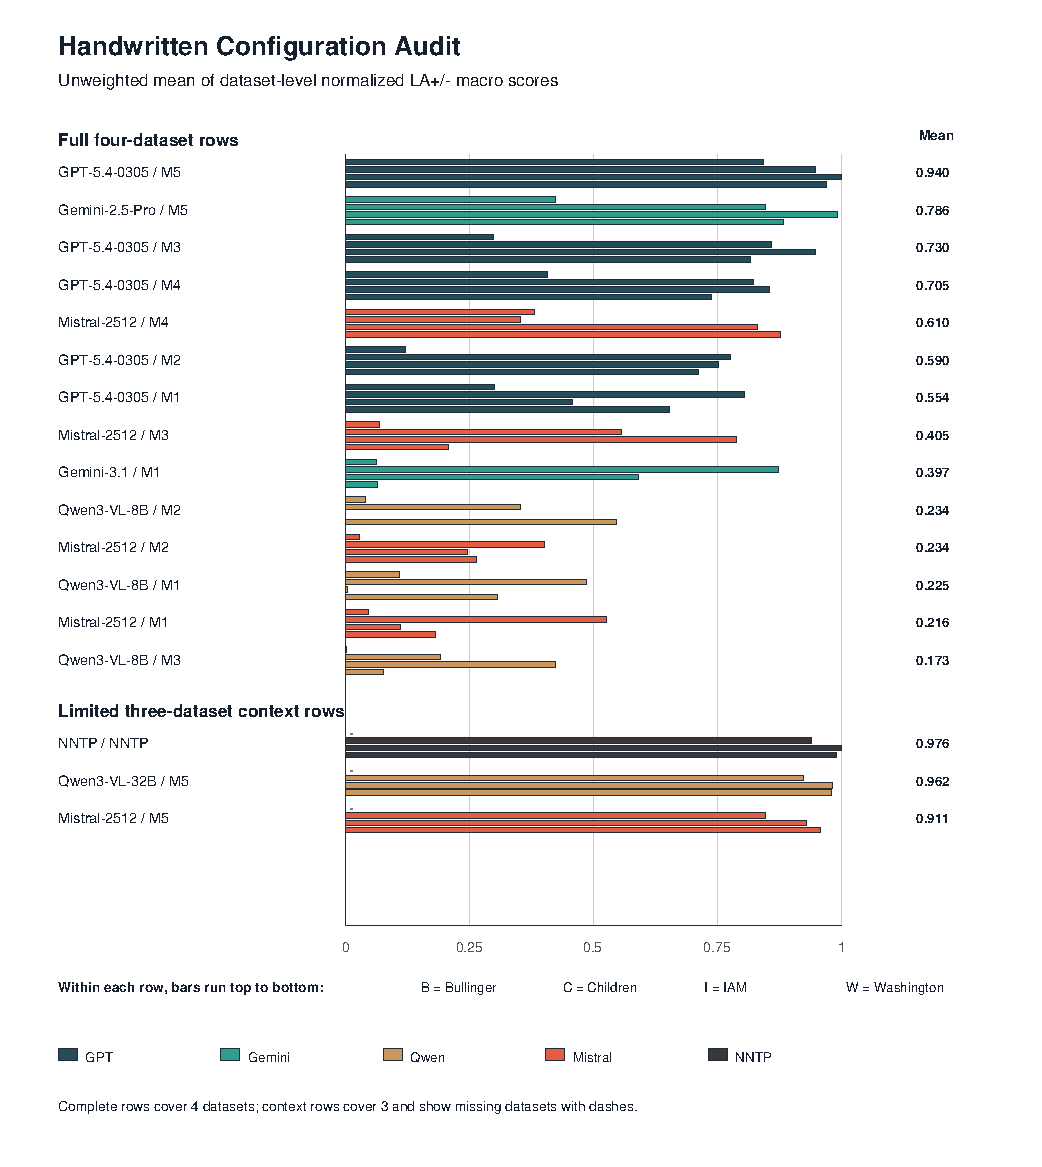
\includegraphics[width=0.98\linewidth,height=0.78\textheight,keepaspectratio]{images/ch6_results/handwritten_model_method_line_accuracy.pdf}
  \caption{Configuration audit of evaluated handwritten model/method runs. Within each row, the bars report dataset-level \LANormCombined{} macro scores in the order Bullinger, Children, IAM, and Washington; dashes mark unavailable datasets in limited context rows. The rightmost mean is the unweighted average of the represented dataset cells and is used only to order the figure. The upper block contains complete four-dataset rows, whereas the lower block contains limited three-dataset context rows. The figure summarizes configuration coverage and context; limited-coverage rows are interpreted through the caveats in the surrounding text and Appendix Table~\ref{tab:app_handwritten_model_method_overview_values}. Table~\ref{tab:exp_handwritten_main_overview} and Table~\ref{tab:exp_handwritten_controlled_model} provide the main LLM/VLM method-configuration comparisons.}
  \label{fig:exp_handwritten_llm_model_overview}
\end{figure}
\FloatBarrier

Table~\ref{tab:exp_handwritten_main_overview} condenses the LLM/VLM side of the same evidence by reporting the highest-scoring complete evaluated row for each dataset and method. This table answers RQ1 at the method-configuration level. Within the reported handwritten evaluation, M5 has the highest observed LLM/VLM macro score for Bullinger Handwritten, Children Handwritten, IAM Handwritten, and Washington Handwritten. The largest reported separation appears on Bullinger, where the M5 setup is far above the raw-output methods. IAM shows a different pattern, because OCR-conditioned M3 is already strong, and M5 reaches the ceiling.

\begin{table}[H]
  \centering
  \caption{Descriptive best-row overview for the four handwritten LLM/VLM-based datasets. Each cell reports \LANormCombined{}, the whitespace-normalized combined order-sensitive line accuracy, macro-averaged over sample IDs and formed as the mean of \LANormForward{} and \LANormReverse{} before rounding. Each dataset-method cell uses the highest-scoring complete row within the handwritten evaluation scope. The table is a descriptive overview, not an ablation or causal method ranking, because model configurations may differ across cells and the structured M4/M5 regimes include stored line-count access, repair, fallback, and projection.}
  \label{tab:exp_handwritten_main_overview}
  \footnotesize
  \setlength{\tabcolsep}{4pt}
  \renewcommand{\arraystretch}{1.08}
  \begin{tabular}{@{}l c c c c c c@{}}
    \toprule
    \textbf{Dataset} & \textbf{\(n\)} & \textbf{M1} & \textbf{M2} & \textbf{M3} & \textbf{M4} & \textbf{M5} \\
    \midrule
    Bullinger Handwritten & 59 & 0.300 & 0.120 & 0.297 & 0.406 & \textbf{0.843} \\
    Children Handwritten & 63 & 0.872 & 0.777 & 0.859 & 0.822 & \textbf{0.948} \\
    IAM & 20 & 0.589 & 0.752 & 0.948 & 0.855 & \textbf{1.000} \\
    Washington Handwritten & 20 & 0.653 & 0.711 & 0.817 & 0.883 & \textbf{0.980} \\
    \bottomrule
  \end{tabular}
  \vspace{0.35em}

  \parbox{0.82\linewidth}{\footnotesize Bold marks the highest value within each dataset row; it does not imply causal attribution. \autoref{sec:appendix_provider_mix} lists the contributing model configurations, and Table~\ref{tab:app_model_provider_aliases} centralizes the display-name aliases. The partial Bullinger \QwenThirtyTwoShort{} M5 row covers \(20/59\) samples because the university-cluster run exhausted GPU memory on larger Bullinger samples. It is preserved as an execution record, but excluded from the complete-dataset comparison and from highest-row conclusions.}
\end{table}

The result should therefore be read as the main M5 finding rather than as evidence for a monotonic method ladder. M5 combines ordered line-image evidence, OCR/HTR line text, page context, structured output, validation, and projection. The current experiments report this setup as the highest-scoring evaluated LLM/VLM-based alignment setup; they do not isolate any single component as the sole cause of the observed differences. The controlled OpenAI table below preserves the same M5 result while reducing model-configuration variation, and \autoref{sec:appendix_prompt_detail_metrics} expands the same rows with directional scores and supporting diagnostics.

The next layer narrows the comparison level. Table~\ref{tab:exp_handwritten_controlled_model} asks whether the same main result remains visible when one OpenAI model configuration is held fixed across M1--M5.

\paragraph{Controlled LLM/VLM-based checks.}
\label{sec:experimentation_controlled_checks}

Table~\ref{tab:exp_handwritten_controlled_model} is the controlled OpenAI comparison for RQ1 because it keeps the LLM/VLM side on a single complete OpenAI model configuration while preserving the five-method progression. Its purpose is not to replace the overview. It tests whether the main result remains visible after one major source of variation is removed.

\begin{table}[H]
  \centering
  \caption{Exact-model OpenAI control for the handwritten LLM/VLM-based comparison. Each cell reports \LANormCombined{}, the whitespace-normalized combined order-sensitive line accuracy, macro-averaged over sample IDs and formed as the mean of \LANormForward{} and \LANormReverse{} before rounding. All rows use \GPTFiveMarchShort{}. The structured M4 and M5 rows retain the known-count prerequisite and projection as part of the evaluated regime.}
  \label{tab:exp_handwritten_controlled_model}
  \footnotesize
  \begin{tabular}{@{}l c c c c c c@{}}
    \toprule
    \textbf{Dataset} & \textbf{Coverage} & \textbf{M1} & \textbf{M2} & \textbf{M3} & \textbf{M4} & \textbf{M5} \\
    \midrule
    Bullinger Handwritten & 59/59 & 0.300 & 0.120 & 0.297 & 0.406 & \textbf{0.843} \\
    Children Handwritten & 63/63 & 0.804 & 0.777 & 0.859 & 0.822 & \textbf{0.948} \\
    IAM & 20/20 & 0.458 & 0.752 & 0.948 & 0.855 & \textbf{1.000} \\
    Washington Handwritten & 20/20 & 0.653 & 0.711 & 0.817 & 0.737 & \textbf{0.970} \\
    \bottomrule
  \end{tabular}
  \vspace{0.35em}

  \parbox{0.82\linewidth}{\footnotesize Bold marks the highest value within each dataset row; it does not imply causal attribution. The M5 column uses the documented zero-shot context-rich M5 configuration. This table is the primary controlled LLM/VLM-based comparison because it keeps one OpenAI model configuration across M1--M5 and uses the full sample set for all four handwritten datasets; the archived M5 OpenAI shorthand is documented in Table~\ref{tab:app_model_provider_aliases}.}
\end{table}

The control table preserves the main result while changing the story about the path to it. Under the \GPTFiveMarchShort{} model configuration, the intermediate steps are clearly non-monotonic. Children drops from \(0.859\) at M3 to \(0.822\) at M4, and Washington drops from \(0.817\) at M3 to \(0.737\) at M4 before jumping to \(0.970\) at M5. Bullinger likewise shows a substantially higher M5 score, but not a smooth method ladder, since the sequence rises from \(0.120\) at M2 to \(0.297\) at M3, \(0.406\) at M4, and \(0.843\) at M5. The supported claim is therefore not monotonicity at every step; it is the specific observation that M5 has the highest observed macro score among the evaluated LLM/VLM-based methods under one OpenAI model configuration across all four datasets.

\paragraph{Takeaway.}
The handwritten tables support a narrow but consistent reading in which M5 is the highest LLM/VLM-based row in both the descriptive overview and the exact-model OpenAI control, while the order of M1--M4 changes by dataset. The tables therefore support M5 as the main result for the reported setups, not a smooth stepwise improvement claim across all methods.

\paragraph{Preliminary check: Adding one example to the prompt.}\label{sec:experimentation_one_shot_exploratory}\mbox{}\par

Before fixing the final handwritten evaluation setup, a small exploratory run tested whether the raw-output methods M1--M3 benefit from one worked example in the prompt. In this setting, each target sample was preceded by one example from the same dataset. This is often called one-shot prompting: The model receives one demonstration of the desired input-output behavior before solving the current sample.

The check was limited to GPT-5.2 and Qwen3-VL-8B and to the early M1--M3 setup. It was not run for M4 or M5 and is not part of the main M1--M5 result claims. Figure~\ref{fig:exp_one_shot_deltas} reports the change from the corresponding zero-example prompt to the one-example prompt. Positive values mean that the one-example prompt improved whitespace-normalized \LANormCombined{}; negative values mean that it reduced accuracy.

\begin{figure}[H]
  \centering
  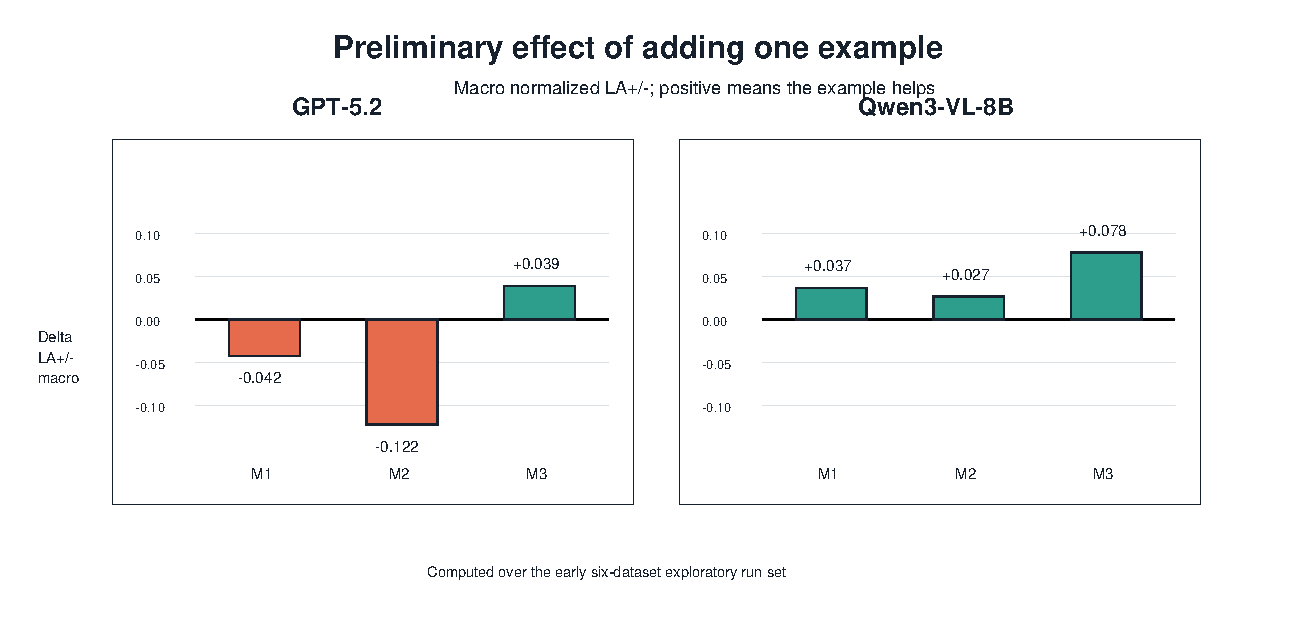
\includegraphics[width=0.88\linewidth]{images/ch6_results/exploratory_one_shot_deltas.pdf}
  \caption{Preliminary effect of adding one worked example to M1--M3 prompts. Bars show the change in whitespace-normalized \LANormCombined{} relative to the corresponding zero-example prompt for two model configurations in an early exploratory run set. Positive values indicate higher line accuracy with the example included. The check is diagnostic only and is not used in the main M1--M5 comparison.}
  \label{fig:exp_one_shot_deltas}
\end{figure}

The result is mixed. The GPT-5.2 row loses accuracy for M1 and M2 but improves for M3, while the \QwenEightShort{} row improves on all three methods from a lower early baseline. This was not a stable enough signal to justify expanding one-example prompting to the structured M4/M5 experiments. The main experiments therefore focus on the final zero-shot and context-rich structured configurations.

\subsection{Model-Configuration Robustness}
\label{sec:experimentation_provider_model_robustness}

The main RQ1 pattern survives the primary complete model-configuration control, where M5 remains the highest-scoring reported LLM/VLM-based configuration while the intermediate rankings stay model- and dataset-sensitive. This robustness check is a guardrail around the first empirical layer. Table~\ref{tab:exp_handwritten_main_overview} and the appendix duplicate in Table~\ref{tab:exp_handwritten_prompt_matrix} are descriptive because each dataset-method cell may be supplied by a different model configuration; the provenance is explicit in Table~\ref{tab:app_handwritten_prompt_provenance}, with display-name aliases centralized in Table~\ref{tab:app_model_provider_aliases}. Table~\ref{tab:exp_handwritten_controlled_model} is the primary controlled LLM/VLM progression table: It keeps one OpenAI model configuration, \GPTFiveMarchShort{}, across M1--M5 and uses the full sample set for all four handwritten datasets. The \MistralLargeShort{} matrix in Table~\ref{tab:app_mistral_fixed_provider_matrix} is stricter in provider scope, but secondary for the thesis argument because its Bullinger M5 cell is missing after the Bullinger M5 run did not complete following API errors and its absolute scores differ from the OpenAI/Qwen/Gemini rows included in the thesis evidence.

Within those results, Washington is the clearest model-sensitive case. The Washington M4 and M5 cells in Table~\ref{tab:exp_handwritten_main_overview} are supplied by \QwenEightShort{} and \QwenThirtyTwoShort{}, with \LANormCombined{} values of \(0.883\) and \(0.980\), whereas the exact OpenAI control reports \(0.737\) for M4 and \(0.970\) for M5 on the same dataset. This does not rank Qwen against OpenAI in general; it shows specifically that the selected Washington results for M4/M5 depend on the selected model configuration. The main conclusion survives the complete OpenAI control, and M5 remains the highest-scoring reported LLM/VLM-based configuration in Table~\ref{tab:exp_handwritten_controlled_model}. The intermediate order of M1--M4 remains model- and dataset-sensitive, so the thesis treats those rankings as contextual rather than as model-family effects isolated from provider and dataset variation.

\FloatBarrier

\section{Secondary Printed-Context Results}
\label{sec:experimentation_print_results}

The secondary printed context provides supporting modality evidence without changing the main handwritten answer. It extends the same newline-only evaluation target to Bullinger Print and IAM Print for the raw-output M1--M3 configurations. Because M4, M5, and NNTP were not run on the printed datasets, this section reports limited M1--M3 rows as secondary printed context rather than a full evidence-and-control progression.

\begin{table}[H]
  \centering
  \caption{Secondary printed-dataset results for the reported M1--M3 scope. Values are whitespace-normalized \LANormCombined{} macro-averages over sample IDs, reported from retained print evaluation CSV macro rows and rounded to three decimals. Each cell reports the highest-scoring complete zero-shot row for that printed dataset and method. M4, M5, and NNTP were not run on the printed datasets and are therefore not shown.}
  \label{tab:exp_print_secondary}
  \footnotesize
  \renewcommand{\arraystretch}{1.08}
  \begin{tabular}{@{}l c c c c@{}}
    \toprule
    \textbf{Dataset} & \textbf{Samples} & \textbf{M1} & \textbf{M2} & \textbf{M3} \\
    \midrule
    Bullinger Print & 10 & \textbf{0.594} (GPT-5.2) & 0.566 (GPT-5.2) & 0.115 (\MistralLargeShort{}) \\
    IAM Print & 30 & 0.917 (GPT-5.2) & 0.896 (GPT-5.2) & \textbf{0.934} (GPT-5.2) \\
    \bottomrule
  \end{tabular}
  \vspace{0.35em}

  \parbox{0.74\linewidth}{\footnotesize Bold marks the highest value within each dataset row.}
\end{table}

The two print datasets behave differently. On IAM Print, the highest stored row is already high for all three raw-output configurations, and the highest M3 row reaches \(\LANormCombinedToken=0.934\), \(\LineFOneNormToken=0.945\), and \(\CERNormToken=0.001\). Bullinger Print is lower and less stable: Its highest M1 and M2 rows reach \(\LANormCombinedToken=0.594\) and \(0.566\), while its highest M3 row falls to \(0.115\) despite \(\CERNormToken=0.009\). This reinforces the line-structure-first reading of the metric stack: Character preservation or low CER does not by itself imply that newline boundaries have been recovered well. Because the print scope lacks M4, M5, and NNTP, these rows broaden modality context but do not change the handwritten conclusion that M5 has the highest reported macro score among the evaluated LLM/VLM-based configurations in the complete main evaluation.

To compare print and handwriting without changing the main handwritten sample sets, Table~\ref{tab:exp_print_handwriting_matched_support} uses restricted support slices in which corresponding print and handwritten rows were reported. These support slices are separate from the main handwritten evaluation sets, including the representative-20 IAM Handwritten main evaluation. The table is therefore diagnostic: It compares modalities within paired support slices and does not replace the main handwritten results in Table~\ref{tab:exp_handwritten_main_overview}.

\begin{table}[H]
  \centering
  \caption{Diagnostic matched-support print--handwriting comparison for M1--M3. Values are whitespace-normalized \LANormCombined{} macro-averages over the restricted support IDs and rounded to three decimals. The support-slice denominators are \(n=10\) shared Bullinger IDs and \(n=30\) paired IAM \texttt{a01-*} forms. The table is a direct comparison within the paired support slices; it does not replace the headline handwritten sample sets used in Table~\ref{tab:exp_handwritten_main_overview}.}
  \label{tab:exp_print_handwriting_matched_support}
  \footnotesize
  \setlength{\tabcolsep}{4pt}
  \renewcommand{\arraystretch}{1.10}
  \begin{tabular}{@{}l c c c c c c@{}}
    \toprule
    \textbf{Dataset} & \shortstack{\textbf{M1}\\\textbf{handwritten}} & \shortstack{\textbf{M1}\\\textbf{print}} & \shortstack{\textbf{M2}\\\textbf{handwritten}} & \shortstack{\textbf{M2}\\\textbf{print}} & \shortstack{\textbf{M3}\\\textbf{handwritten}} & \shortstack{\textbf{M3}\\\textbf{print}} \\
    \midrule
    Bullinger & 0.148 & 0.594 & 0.083 & 0.566 & 0.066 & 0.115 \\
    IAM & 0.959 & 0.917 & 0.912 & 0.896 & 0.802 & 0.934 \\
    \bottomrule
  \end{tabular}
\end{table}

The diagnostic comparison separates two patterns. For Bullinger, print scores higher than the matched handwritten support slice for M1--M3, but Bullinger Print M3 remains much lower than Bullinger Print M1 and M2. For IAM, both modalities are strong; IAM Print peaks at M3, while the matched IAM Handwritten support remains high but peaks earlier. Since M4, M5, and NNTP were not run for the secondary printed context datasets, this direct M1--M3 comparison does not test the full evidence-and-control progression used in the main handwritten evaluation.

\FloatBarrier

\section{Comparison with NNTP}
\label{sec:experimentation_direct_nntp}

RQ2 has a close, dataset-dependent answer rather than a uniform winner. On the three datasets with thesis-side dataset-level NNTP summaries over the same sample sets, M5 is slightly ahead on Children Handwritten, tied on IAM Handwritten, and slightly behind on Washington Handwritten. Table~\ref{tab:exp_best_vs_nntp} is therefore the same-sample thesis-side comparison for Children, IAM, and Washington. Bullinger is treated separately because its deterministic comparison is made against the published Bullinger alignment baseline rather than against a full \(59\)-sample thesis-side NNTP run.

\begin{table}[H]
  \centering
  \caption{Same-sample NNTP comparison for Children, IAM, and Washington. Values are whitespace-normalized \LANormCombined{} macro-averages over sample IDs. LLM/VLM rows use the highest-scoring complete reported M5 row per dataset; NNTP rows are thesis-side summaries or the legacy IAM run.}
  \label{tab:exp_best_vs_nntp}
  \footnotesize
  \renewcommand{\arraystretch}{1.08}
  \begin{tabularx}{\linewidth}{@{}Y c Y c Y c c@{}}
    \toprule
    \textbf{Dataset} & \textbf{Samples} & \textbf{LLM/VLM} & \(\mathbf{\LANormCombinedToken}\) & \textbf{NNTP setup} & \(\mathbf{\LANormCombinedToken}\) & \(\mathbf{\Delta}\) \\
    \midrule
    Children Handwritten & 63 & M5 / \GPTFiveShort{} & \textbf{0.948} & cross-validation macro (3-fold) & 0.939 & +0.009 \\
    IAM & 20 & M5 / \GPTFiveShort{} & \textbf{1.000} & legacy single run & \textbf{1.000} & 0.000 \\
    Washington Handwritten & 20 & M5 / \QwenThirtyTwoShort{} & 0.980 & cross-validation macro (2-fold) & \textbf{0.990} & -0.009 \\
    \bottomrule
  \end{tabularx}
  \vspace{0.35em}

  \parbox{0.96\linewidth}{\footnotesize Bold marks the higher value within each dataset row; ties bold both values. It is not a significance claim. Paired sample-level reconstruction gives Children \(4\) LLM/VLM wins, \(2\) NNTP wins, \(57\) ties, and \(6\) non-tied pairs; IAM \(0\) wins for either side, \(20\) ties, and \(0\) non-tied pairs; and Washington \(2\) LLM/VLM wins, \(4\) NNTP wins, \(14\) ties, and \(6\) non-tied pairs. NNTP aligns recognizer labels after symbol-inventory preprocessing rather than the untouched transcription.}
\end{table}

The comparison is direct in its metric target because both sides are scored as newline-only line reconstructions, while the implemented regimes differ. M5 uses prompts, structured controls, and projection that can restore the fixed transcription before scoring, whereas NNTP searches a forced-alignment path over recognizer-derived CTC evidence rather than producing free-form text \thesiscite{peer2025ctcBullingerAlignment}. With the preprocessing limit recorded in the table note, line accuracy is the main shared surface; character-level readings against M1--M5 retain the NNTP symbol-filtering condition summarized in Table~\ref{tab:app_nntp_symbol_filter_audit}.

At sample level, the comparison is dominated by ties. Children has 4 LLM/VLM wins, 2 NNTP wins, and 57 ties; IAM has 20 ties; Washington has 2 LLM/VLM wins, 4 NNTP wins, and 14 ties. The few non-tied cases do not support a directional claim. A two-sided exact sign test gives \(p = 0.688\) for Children (\(4\) vs.\ \(2\), \(n=6\) non-tied pairs) and \(p = 0.688\) for Washington (\(2\) vs.\ \(4\), \(n=6\) non-tied pairs), while IAM has no non-tied pairs to test. The sample-level evidence therefore supports closeness and tie-dominance rather than a clear advantage for either approach.

\paragraph{Takeaway.}
The same-sample NNTP comparison is close rather than one-sided. On the matched handwritten comparison sets, Children slightly favors M5, IAM ties, and Washington slightly favors NNTP; the paired counts are dominated by ties. Bullinger is outside this matched claim except for the subset-level context below. Within this comparison, the evidence supports a close, tie-dominated, and dataset-dependent RQ2 interpretation.

\FloatBarrier

\paragraph{Bullinger published-baseline context.}
\label{sec:experimentation_bullinger_contextual}

Bullinger remains part of the NNTP discussion because the recent Bullinger alignment study reports a deterministic baseline for the same task family \thesiscite{peer2025ctcBullingerAlignment}. Unlike Children, IAM, and Washington, the comparison is not a full thesis-side NNTP run over the \(59\)-sample thesis denominator. It is a subset-level comparison against the published Bullinger baseline.

Table~\ref{tab:exp_bullinger_contextual} reports this comparison using raw forward line accuracy \(\LAForward\) to stay close to the published baseline. Subset~1 is directly comparable because the thesis subset matches the published inventory at the letter and line level. Subset~2 is contextual because the thesis and paper inventories differ.

\begin{table}[t]
  \centering
  \caption{Bullinger published-baseline comparison against the published NNTP baseline. Values are raw \LAForward{} scores, not whitespace-normalized \LANormForward{} scores; thesis-side values are macro-averaged over sample IDs, while the paper values are the published subset-level NNTP scores. All thesis-side Bullinger runs use the same author-provided subset version; direct comparison to the paper is possible for Subset~1 but remains contextual for Subset~2.}
  \label{tab:exp_bullinger_contextual}
  \footnotesize
  \renewcommand{\arraystretch}{1.08}
  \begin{tabularx}{\linewidth}{@{}Y c Y c c c@{}}
    \toprule
    \textbf{Subset} & \textbf{Thesis sample set} & \textbf{Highest-scoring thesis LLM/VLM configuration} & \(\mathbf{\LAForwardToken}\) & \textbf{Paper sample set} & \(\mathbf{\LAForwardToken}\) \\
    \midrule
    Subset~1 & 20 letters / 902 lines & M5 / \GPTFiveShort{} & 0.821 & 20 letters / 902 lines & \textbf{0.861} \\
    Subset~2 & 39 letters / 1633 lines & M5 / \GPTFiveShort{} & \textbf{0.865} & 49 letters / 1486 lines & 0.773 \\
    \bottomrule
  \end{tabularx}
  \vspace{0.35em}

  \parbox{0.96\linewidth}{\footnotesize Bold marks the higher \LAForward{} value within each subset row. Subset~1 is direct because it matches at the letter and line level; Subset~2 is contextual because the thesis and paper inventories differ.}
\end{table}

\FloatBarrier

The result is mixed in a precise way. On Subset~1, the published NNTP result is higher than the thesis M5 result. On Subset~2, the thesis M5 value is higher, but this comparison is contextual because the inventories differ. The Bullinger evidence therefore does not support a single full-dataset M5-versus-NNTP winner. It shows that NNTP remains stronger on the directly matched subset, while M5 is higher only in the contextual Subset~2 comparison \thesiscite{peer2025ctcBullingerAlignment}.

\section{Output Control and Fixed-Transcription Validity}
\label{sec:experimentation_output_control_audit}

RQ3 asks a validity question before an accuracy question. The central issue is whether the scored output is a newline plan over the supplied transcription rather than a generated transcription. The structured M5 traces show that this control path works reliably in the archived context-rich handwritten runs. Across \(162/162\) samples, the first strict JSON response already satisfied the exact-count requirement for \(157\) samples. The remaining cases were handled by the repair, loose-recovery, or deterministic-fallback paths; all such events occur in Bullinger. After the selected boundary plan is projected onto the untouched transcription, the final scored string preserves the fixed character stream.

Table~\ref{tab:app_m5_trace_event_counts} gives the corresponding M5 event-count audit by dataset and explains how M5 combines generative evidence with fixed-transcription validity: Model-proposed lines are treated as boundary evidence, not as final text.

\begin{table}[H]
  \centering
  \caption{Structured output-validity events archived for the complete \GPTFiveShort{} context-rich M5 configuration in the reported handwritten evaluation set. These are event counts rather than whitespace-normalized metric values or sample-ID macro-averages.}
  \label{tab:app_m5_trace_event_counts}
  \footnotesize
  \renewcommand{\arraystretch}{1.08}
  \begin{tabular}{@{}l c c c c c c c c@{}}
    \toprule
    \textbf{Dataset} & \textbf{Samples} & \shortstack{\textbf{1st}\\\textbf{JSON}} & \textbf{Repair} & \textbf{Loose} & \textbf{Fallback} & \shortstack{\textbf{Final proj.}\\\textbf{mode}} & \textbf{Fail} & \textbf{Missing} \\
    \midrule
    Bullinger Handwritten & 59 & 54 & 2 & 3 & 3 & 39 & 0 & 0 \\
    Children Handwritten & 63 & 63 & 0 & 0 & 0 & 58 & 0 & 0 \\
    IAM (20-form) & 20 & 20 & 0 & 0 & 0 & 20 & 0 & 0 \\
    Washington Handwritten & 20 & 20 & 0 & 0 & 0 & 19 & 0 & 0 \\
    \bottomrule
  \end{tabular}
  \vspace{0.35em}

  \parbox{0.88\linewidth}{\footnotesize\raggedright ``1st JSON'' counts samples whose first strict parse already satisfied the exact-count JSON requirement. ``Repair'' counts samples whose first strict parse failed but whose repair response then succeeded. ``Loose'' counts traces that recovered a usable boundary plan from non-strict model lines (\texttt{reconciled\_model\_lines} or \texttt{quality\_repair\_recovered}). ``Fallback'' marks deterministic fallback projection. ``Final proj. mode'' counts traces whose final logged resolution mode is \texttt{projection\_from\_model\_lines}; candidate projections evaluated inside \texttt{reference\_alignment\_selection} are not exposed as a separate boolean in the stored schema and are therefore not double-counted here. ``Missing'' \(=0\) indicates complete trace availability for this M5 audit layer. The event columns are trace flags rather than a mutually exclusive partition of samples; a sample may satisfy more than one condition, for example by parsing successfully and still being projected, or by passing through repair before fallback. More broadly, the M5 scored string is not raw returned text: Accepted, recovered, or fallback boundary plans may be projected back onto the untouched transcription before evaluation.}
\end{table}
\FloatBarrier

The event-count audit is reported for M5 because the final structured M5 runs have complete trace records for the handwritten evaluation. M4 follows the same structured-output principle and remains part of the score tables, but its trace records are not complete enough for a parallel event-count summary. The M5 event counts should therefore be read as evidence for the final structured configuration, not as inferred totals for M4.

The same distinction is visible in a simpler line-count diagnostic. Before asking whether a boundary is placed exactly, Table~\ref{tab:exp_line_count_drift} asks whether the output has the right number of lines at all. For each LLM/VLM scored prediction, \(\Delta L\) is defined as the number of predicted lines minus the number of ground truth lines after splitting the prediction and ground truth text on newlines; \MeanAbsLineDelta{} denotes the corresponding mean absolute line-count difference. The table reports all canonical scored rows for which prediction and ground truth text could both be reconstructed; this set is complete for the scored rows included here (\(2633/2633\)).

\begin{table}[H]
  \centering
  \caption{Line-count drift in documented handwritten LLM/VLM rows. This is not a whitespace-normalized accuracy table: Predicted and ground truth line counts are summed over scored rows whose prediction and ground truth text could both be reconstructed, repeated samples across model configurations remain separate observations, and \MeanAbsLineDelta{} is averaged over those rows rather than macro-averaged over unique sample IDs.}
  \label{tab:exp_line_count_drift}
  \footnotesize
  \renewcommand{\arraystretch}{1.08}
  \begin{tabular}{@{}l c r r c r r r@{}}
    \toprule
    \textbf{Method} & \textbf{Rows} & \textbf{Pred. lines} & \textbf{GT lines} & \(\mathbf{\MeanAbsLineDeltaToken}\) & \(\mathbf{\Delta L=0}\) & \textbf{Under} & \textbf{Over} \\
    \midrule
    M1 & 648/648 & 10894 & 15060 & 7.630 & 275 & 295 & 78 \\
    M2 & 506/506 & 9570 & 11951 & 5.911 & 244 & 197 & 65 \\
    M3 & 506/506 & 6334 & 11951 & 11.204 & 218 & 271 & 17 \\
    M4 & 423/423 & 10848 & 10901 & 0.125 & 399 & 24 & 0 \\
    M5 & 550/550 & 10426 & 10430 & 0.007 & 546 & 4 & 0 \\
    \bottomrule
  \end{tabular}
  \vspace{0.35em}

  \parbox{0.96\linewidth}{\footnotesize Under and over count rows with fewer or more predicted lines than the ground truth. Aggregated across methods, the raw-output rows M1--M3 have \MeanAbsLineDelta{} \(=8.195\) over \(1660\) rows, whereas the structured rows M4--M5 have \MeanAbsLineDelta{} \(=0.059\) over \(973\) rows.}
\end{table}

Table~\ref{tab:exp_line_count_drift} supports RQ3 as output-validity evidence rather than as an independent accuracy claim. M1--M3 frequently under-segment or over-segment because the raw returned text must both copy the transcription and choose the global number of output lines. Reliable ordered line metadata is an operational prerequisite of M4/M5 as evaluated, and their configurations validate against the stored cardinality before repairing, recovering, falling back, or projecting before scoring. In the handwritten datasets used here, the stored \texttt{ocr\_lines} cardinality matches the ground-truth line count, so the structured configurations test boundary assignment under known-count staging rather than blind line-count prediction. Their low \MeanAbsLineDelta{} should therefore be interpreted as output validity under that condition, not as evidence of page-side line-count inference.

This analysis also defines the scope of the RQ3 evidence. The equivalent M4 event-count trace layer is incomplete: The appendix documents the M4 control logic, but not same-sample M4 event totals across the handwritten datasets. M4 event totals are therefore not reported from traces, and they should not be inferred from the M5 layer or from code-level behavior alone. Consequently, Chapter~7 can answer RQ3 at the configuration and output-validity level: Structured output control is practically important because it makes the scored LLM/VLM outputs valid under the fixed-transcription newline-only task definition. Isolated effects of strict JSON, repair, fallback, and projection remain future ablation questions because those controls co-vary with the known-count staging, evidence scaffolds, crop provenance, and provider behavior.

\paragraph{Takeaway.}
The output-control evidence shows a validity difference before it shows an accuracy difference: M1--M3 often return the wrong number of lines, whereas M4 and M5 are evaluated after exact-count validation, possible repair or fallback, and projection under known-count staging. This supports the fixed-transcription validity claim for the structured configurations, with component-level attribution left to targeted ablation work.

\section{Qualitative Error Analysis}
\label{sec:experimentation_qualitative}

The final empirical layer moves from score tables to prediction-level mechanisms. It does not replace the aggregate tables; it explains why their patterns are plausible by tracing how line-count drift, positional shifts, OCR noise, structured fallback, and NNTP local boundary choices appear in stored predictions.

\FloatBarrier

\subsection{Method-Level Error Mechanisms}
\label{sec:experimentation_method_weaknesses}

The mechanism-level reading is that the configurations fail for different reasons, so the aggregate RQ answers should be read as configuration-level evidence rather than as isolated component effects. The prediction- and trace-level analysis of stored artifacts turns the preceding score differences into method-level mechanisms. Table~\ref{tab:exp_method_weakness_mechanisms} is the analytical bridge between aggregate scores and individual excerpts: It reads each row through the same questions--what helps, what fails, which mechanism is visible, and how that mechanism bounds the research-question answer. Appendix Table~\ref{tab:app_method_weakness_evidence} keeps the counted rows, named sample IDs, trace evidence, and longer mechanism notes that support this compact reading. The main-text table therefore summarizes secondary analysis of stored artifacts; appendix counts support traceability, while named samples remain illustrative rather than prevalence estimates.

\begin{table}[!htbp]
  \centering
  \caption{Analytical summary of observed method strengths, limitations, and likely error mechanisms in the documented prediction- and trace-level analysis. Appendix Table~\ref{tab:app_method_weakness_evidence} preserves the counted evidence, sample IDs, trace details, and longer explanations behind these summaries. For NNTP, character-level interpretation preserves the NNTP preprocessing caveat.}
  \label{tab:exp_method_weakness_mechanisms}
  \footnotesize
  \setlength{\tabcolsep}{3pt}
  \renewcommand{\arraystretch}{1.10}
  \begin{tabularx}{\linewidth}{@{}>{\raggedright\arraybackslash}p{0.075\linewidth}>{\raggedright\arraybackslash}p{0.20\linewidth}>{\raggedright\arraybackslash}p{0.21\linewidth}>{\raggedright\arraybackslash}p{0.25\linewidth}Y@{}}
    \toprule
    \textbf{Method} & \textbf{Main strength} & \textbf{Observed limitation} & \textbf{Likely mechanism} & \textbf{Implication} \\
    \midrule
    M1 & Useful when the raw response respects the fixed character stream. & Weak raw-output constraint; omissions, additions, character drift, and count drift. & Copying and segmenting happen in one unconstrained generation; early drift shifts the sequence. & Image evidence helps RQ1 when the fixed-transcription requirement holds; motivates RQ3 control. \\
    \addlinespace[0.35em]
    M2 & OCR/HTR can rescue image-only failures when hint lineation is close. & OCR noise or chunk mismatch can hurt relative to M1. & The model may follow a noisy hint or mispaired chunk over the fixed transcription. & OCR/HTR is a noisy structural hint, not monotonic extra evidence. \\
    \addlinespace[0.35em]
    M3 & Strong when OCR line order is already close to the ground truth. & Cannot correct OCR-side boundary or ordering mistakes; often under-segments. & The text hint can be enough on OCR-friendly pages, but no image signal remains. & Evidence quality matters more than simply adding channels. \\
    \addlinespace[0.35em]
    M4 & Usually controls line count and preserves the transcription after projection. & Correct count can still leave wrong order-sensitive boundaries; not consistently above M3. & Structured OCR scaffolds constrain form but can also lock in flawed OCR splits. & RQ3 validity improves, but RQ1 should not treat M4 as a guaranteed accuracy gain. \\
    \addlinespace[0.35em]
    M5 & Highest reported LLM/VLM macro score overall; projection preserves the fixed stream. & Counterexamples remain around repair, fallback, hyphenation, and short-line anchors. & The evaluated context-rich line-image configuration usually anchors boundaries, but local decisions and trace modes remain entangled. & Supports the highest-scoring evaluated configuration, not an every-sample or component-level causal claim. \\
    \addlinespace[0.35em]
    NNTP & Competitive deterministic forced alignment on matched datasets. & Local merge/split errors remain; character comparison has the preprocessing caveat. & Fixed count and CTC evidence constrain the search, but local boundary placement can still shift. & RQ2 is close and dataset-dependent; line accuracy is primary. \\
    \bottomrule
  \end{tabularx}
\end{table}

Read across the rows, the table gives a compact explanation for the non-monotonic LLM/VLM progression in Tables~\ref{tab:exp_handwritten_main_overview} and~\ref{tab:exp_handwritten_controlled_model}. Extra evidence helps where it is both structurally informative and brought under the fixed-transcription requirement; otherwise it can add a new failure channel. This is why the qualitative analysis first names configuration-level mechanisms and only then turns to individual excerpts.

The M2 pattern explains why adding OCR/HTR hints does not automatically improve M1. In the same-model pairs, M2 is more often worse than better relative to M1, even though individual samples show clear help from OCR/HTR lineation. The mechanism visible in the predictions is not a contradiction: M2 adds a second structural signal but still scores raw returned text, and that signal can be noisy or mismatched to the image/transcription chunk presented to the model. M3 shows the complementary case. When OCR/HTR line order is already close to the ground truth, as in the IAM plateau case, the text-only prompt can recover the lineation without needing page images; when OCR/HTR boundaries are wrong, M3 has no visual fallback.

M4 and M5 separate output validity from boundary accuracy. Two Washington sample IDs are used below as named diagnostic cases. Washington 307 is the case in Table~\ref{tab:exp_f1_la_divergence_cases} where M4 preserves the text but splits the opening header/date in a way that shifts the order-sensitive line sequence. Washington 270 is the case in Table~\ref{tab:exp_linebreak_comparison} where the selected M5 row enters fallback after repair and over-splits the hyphenated \texttt{Recrui-\textbackslash nting} boundary; the matched NNTP row preserves the ground truth split. These cases illustrate sample-level mechanisms and are not prevalence estimates. M4's stronger JSON and line-count scaffold explains why it usually preserves the expected count, but the Washington 307 case shows that a correct count and high exact-line F1 can coexist with order-sensitive failure. M5 adds the evaluated context-rich line-image configuration and has the highest reported overall LLM/VLM macro scores, yet the stored predictions and traces still contain counterexamples. The Washington 270 case shows that the selected M5 row can trail M3 on an individual page. Fallback and repair-attempt trace slices have lower average \LANormCombined{}, and local hyphen or short-line placements remain visible error mechanisms. These trace associations are descriptive because trace mode co-varies with dataset, provider, and sample difficulty.

The NNTP row carries the RQ2 result into the mechanism layer. The same-sample table gives small dataset-level differences, and the paired counts are dominated by ties. Prediction-level evidence explains why: NNTP often has the right line count and stable text-side behavior, but it can still merge two neighboring ground-truth lines or split at the wrong local position. With NNTP-side symbol filtering kept in view, the shared line-accuracy metric family remains the primary comparison level.

\FloatBarrier

\subsection{Excerpt-Backed Qualitative Cases}
\label{sec:experimentation_qualitative_cases}

The excerpt-backed examples narrow the mechanism view to concrete line-break behavior. Their purpose is explanatory: The aggregate tables and paired same-sample NNTP counts carry the average-behavior claims, while the examples show how nearly perfect character preservation can coexist with wrong line structure, why OCR hints can both help and mislead, why IAM can plateau across methods, and how an NNTP-favored Washington case can arise. Each example is anchored by the same per-sample metrics used throughout the chapter, especially \LANormCombined, \LineFOneNorm, and \CERNorm.

A more specific diagnostic split appears when \LineFOneNorm{} and \LANormCombined{} disagree. As defined in \autoref{sec:experimentation_line_alignment_metrics}, normalized exact-line F1 is order-insensitive: It asks whether full normalized ground-truth line strings can be matched somewhere in the prediction. By contrast, \LANormCombined{} is order-sensitive and directional. Table~\ref{tab:exp_f1_la_divergence_cases} is therefore not a gallery of unusual failures; it isolates the metric mechanism behind several aggregate readings. Many line strings can be present as exact strings, but one omitted line or one local split can move the sequence out of positional agreement. These rows explain why the thesis reports both metric families.

\begin{table}[!htbp]
  \centering
  \caption{Diagnostic cases where normalized exact-line F1 is high while normalized bidirectional order-sensitive line accuracy is much lower. Values are whitespace-normalized per-sample metrics, not macro-averages over sample IDs; explanations are based on the corresponding stored predictions and ground-truth texts.}
  \label{tab:exp_f1_la_divergence_cases}
  \footnotesize
  \renewcommand{\arraystretch}{1.12}
  \setlength{\tabcolsep}{3pt}
  \begin{tabularx}{\linewidth}{@{}>{\raggedright\arraybackslash}p{0.15\linewidth}>{\raggedright\arraybackslash}p{0.18\linewidth}c c c Y@{}}
    \toprule
    \textbf{Dataset/sample} & \textbf{Method/model configuration} & \(\mathbf{\LANormCombinedToken}\) & \(\mathbf{\LineFOneNormToken}\) & \(\mathbf{\CERNormToken}\) & \textbf{Mechanism} \\
    \midrule
    Bullinger 12517 & M1 / \GPTFiveMarchShort{} & 0.000 & 0.909 & 0.006 & The opening identifier line is omitted; most remaining line strings still occur, but the prediction begins at the second ground-truth line and never regains positional agreement. \\
    \addlinespace[0.25em]
    Bullinger 11084 & M1 / \GPTFiveMarchShort{} & 0.484 & 0.984 & 0.003 & A single missing opening identifier gives forward accuracy \(0.000\), while reverse accuracy remains \(0.969\) because the tail realigns almost perfectly. \\
    \addlinespace[0.25em]
    Washington 307 & M4 / \GPTFiveMarchShort{} & 0.000 & 0.839 & 0.000 & The structured scaffold splits the opening header/date into separate lines, shifting the following sequence even though most normalized line strings are still recovered. \\
    \addlinespace[0.25em]
    Washington 305 & M3 / \GPTFiveMarchShort{} & 0.485 & 0.985 & 0.002 & The standalone \texttt{GW} line is dropped near the end; nearly all line strings remain, but the suffix is shifted by one line. \\
    \bottomrule
  \end{tabularx}
\end{table}

Table~\ref{tab:exp_f1_la_divergence_cases} isolates the order-sensitive metric contrast. The final qualitative table then broadens from that contrast to the five mechanisms needed for the chapter's argument.

The selected qualitative cases cover content-preserving structural failure, OCR-noise recovery, high exact-line F1 with low line accuracy, plateau or tie behavior, and a boundary case in which the matched M5 row is beaten by NNTP after a logged M5 fallback trace. Table~\ref{tab:exp_linebreak_comparison} is a mechanism guide rather than an appendix substitute: It shows which comparison each case illustrates, which metrics make the mechanism visible, and where the longer excerpt evidence can be checked. Longer line-break excerpts are preserved in Appendix Tables~\ref{tab:app_qualitative_excerpt_blocks} and~\ref{tab:app_qualitative_ocr_excerpt}. Figures~\ref{fig:exp_qualitative_input_washington} and~\ref{fig:exp_qualitative_input_children} show two corresponding source images.

\providecommand{\excerptnl}{\mbox{\texttt{\textbackslash n}}}
\begin{table}[!htbp]
  \centering
  \caption{Analytical guide to the selected qualitative cases. The metrics column uses whitespace-normalized per-sample values, not macro-averages over sample IDs: \LANormCombined{} denotes normalized bidirectional order-sensitive line accuracy, \LineFOneNorm{} denotes normalized exact-line F1, and \CERNorm{} denotes normalized character error rate. Full excerpt blocks with explicit line-break markers are preserved in Appendix Tables~\ref{tab:app_qualitative_excerpt_blocks} and~\ref{tab:app_qualitative_ocr_excerpt}.}
  \label{tab:exp_linebreak_comparison}
  \scriptsize
  \renewcommand{\arraystretch}{1.08}
  \setlength{\tabcolsep}{2pt}
  \begin{tabularx}{\linewidth}{@{}>{\raggedright\arraybackslash}p{0.15\linewidth}>{\raggedright\arraybackslash}p{0.19\linewidth}>{\raggedright\arraybackslash}p{0.34\linewidth}Y@{}}
    \toprule
    \textbf{Dataset/sample} & \textbf{Role} & \textbf{Compared method/model configurations and metrics} & \textbf{Mechanism} \\
    \midrule
    Washington 304 & Content-preserving structural failure & M3 / \GPTFiveMarchShort{}: \(\LANormCombinedToken=0.338\), \(\LineFOneNormToken=0.708\), \(\CERNormToken=0.000\)\par M5 / \GPTFiveShort{}: \(\LANormCombinedToken=1.000\), \(\LineFOneNormToken=1.000\), \(\CERNormToken=0.000\) & M3 preserves the character stream but collapses the opening partition into fewer metric lines; the M5 projection row restores the line count and opening boundaries. \\
    \addlinespace[0.35em]
    Children \texttt{3B\_19\_2-3} & OCR-noise recovery & M2 / \GPTFiveMarchShort{}: \(\LANormCombinedToken=0.286\), \(\LineFOneNormToken=0.286\), \(\CERNormToken=0.190\)\par M3 / \GPTFiveMarchShort{}: \(\LANormCombinedToken=0.714\), \(\LineFOneNormToken=0.714\), \(\CERNormToken=0.164\)\par M5 / \GPTFiveShort{}: \(\LANormCombinedToken=1.000\), \(\LineFOneNormToken=1.000\), \(\CERNormToken=0.000\) & The OCR-conditioned rows lose or normalize the diplomatic \texttt{\&} annotation and related line text; the M5 row projects a line-image boundary plan back onto the fixed transcription. \\
    \addlinespace[0.35em]
    Bullinger 12517 & High exact-line F1 but low line accuracy & M1 / \GPTFiveMarchShort{}: \(\LANormCombinedToken=0.000\), \(\LineFOneNormToken=0.909\), \(\CERNormToken=0.006\)\par M5 / \GPTFiveShort{}: \(\LANormCombinedToken=1.000\), \(\LineFOneNormToken=1.000\), \(\CERNormToken=0.000\) & The M1 row drops the opening identifier line, so many line strings still match as a multiset but the positional line sequence never aligns. \\
    \addlinespace[0.35em]
    IAM \texttt{p06-042} & Plateau / tie behavior & M3 / \GPTFiveMarchShort{}, M4 / \GPTFiveMarchShort{}, M5 / \GPTFiveShort{}, and NNTP / NNTP all report \(\LANormCombinedToken=1.000\), \(\LineFOneNormToken=1.000\), \(\CERNormToken=0.000\). & The OCR-grounded and forced-alignment evidence already matches the ground-truth lineation, so the richer M5 row adds no measurable sample-level gain. \\
    \addlinespace[0.35em]
    Washington 270 & M5 boundary case, NNTP-favored matched case, and documented fallback trace & M3 / \GPTFiveMarchShort{}: \(\LANormCombinedToken=0.935\), \(\LineFOneNormToken=0.935\), \(\CERNormToken=0.002\)\par M5 / \QwenThirtyTwoShort{}: \(\LANormCombinedToken=0.871\), \(\LineFOneNormToken=0.871\), \(\CERNormToken=0.002\); trace \texttt{fallback\_projection} after \texttt{initial+repair}\par NNTP / NNTP: \(\LANormCombinedToken=1.000\), \(\LineFOneNormToken=1.000\), \(\CERNormToken=0.000\) & The selected Washington M5 row locally over-splits hyphenated \texttt{Recrui-\textbackslash nting} as \texttt{Recrui\textbackslash n- ting}; the matched NNTP row keeps the ground-truth split. \\
    \bottomrule
  \end{tabularx}
\end{table}

\FloatBarrier

\paragraph{Content can be correct while line structure is still wrong.}
A central mechanism is content-preserving structural failure. Washington sample 304 is the cleanest illustration of why this thesis separates structural accuracy from character accuracy; it is shown with line overlay in Figure~\ref{fig:exp_qualitative_input_washington}, summarized in the first row of Table~\ref{tab:exp_linebreak_comparison}, and excerpted fully in Appendix Table~\ref{tab:app_qualitative_excerpt_blocks}. On this sample, the selected M3/\GPTFiveMarchShort{} row already achieves \(\CERNormToken=0.000\), but its \LANormCombined{} remains at \(0.338\) and \(\LineFOneNormToken=0.708\); M4/\GPTFiveMarchShort{} rises to \(\LANormCombinedToken=\LineFOneNormToken=0.941\) with \(\CERNormToken=0.000\), and M5 reaches \(\LANormCombinedToken=\LineFOneNormToken=1.000\) with \(\CERNormToken=0.000\). The page therefore reads correctly at the character level long before it is segmented correctly at the line level. This is a case in which the reported structured setups with ordered OCR scaffolds and then line-image anchors improve the line partition, without isolating either evidence source as the sole cause.

\begin{figure}[H]
  \centering
  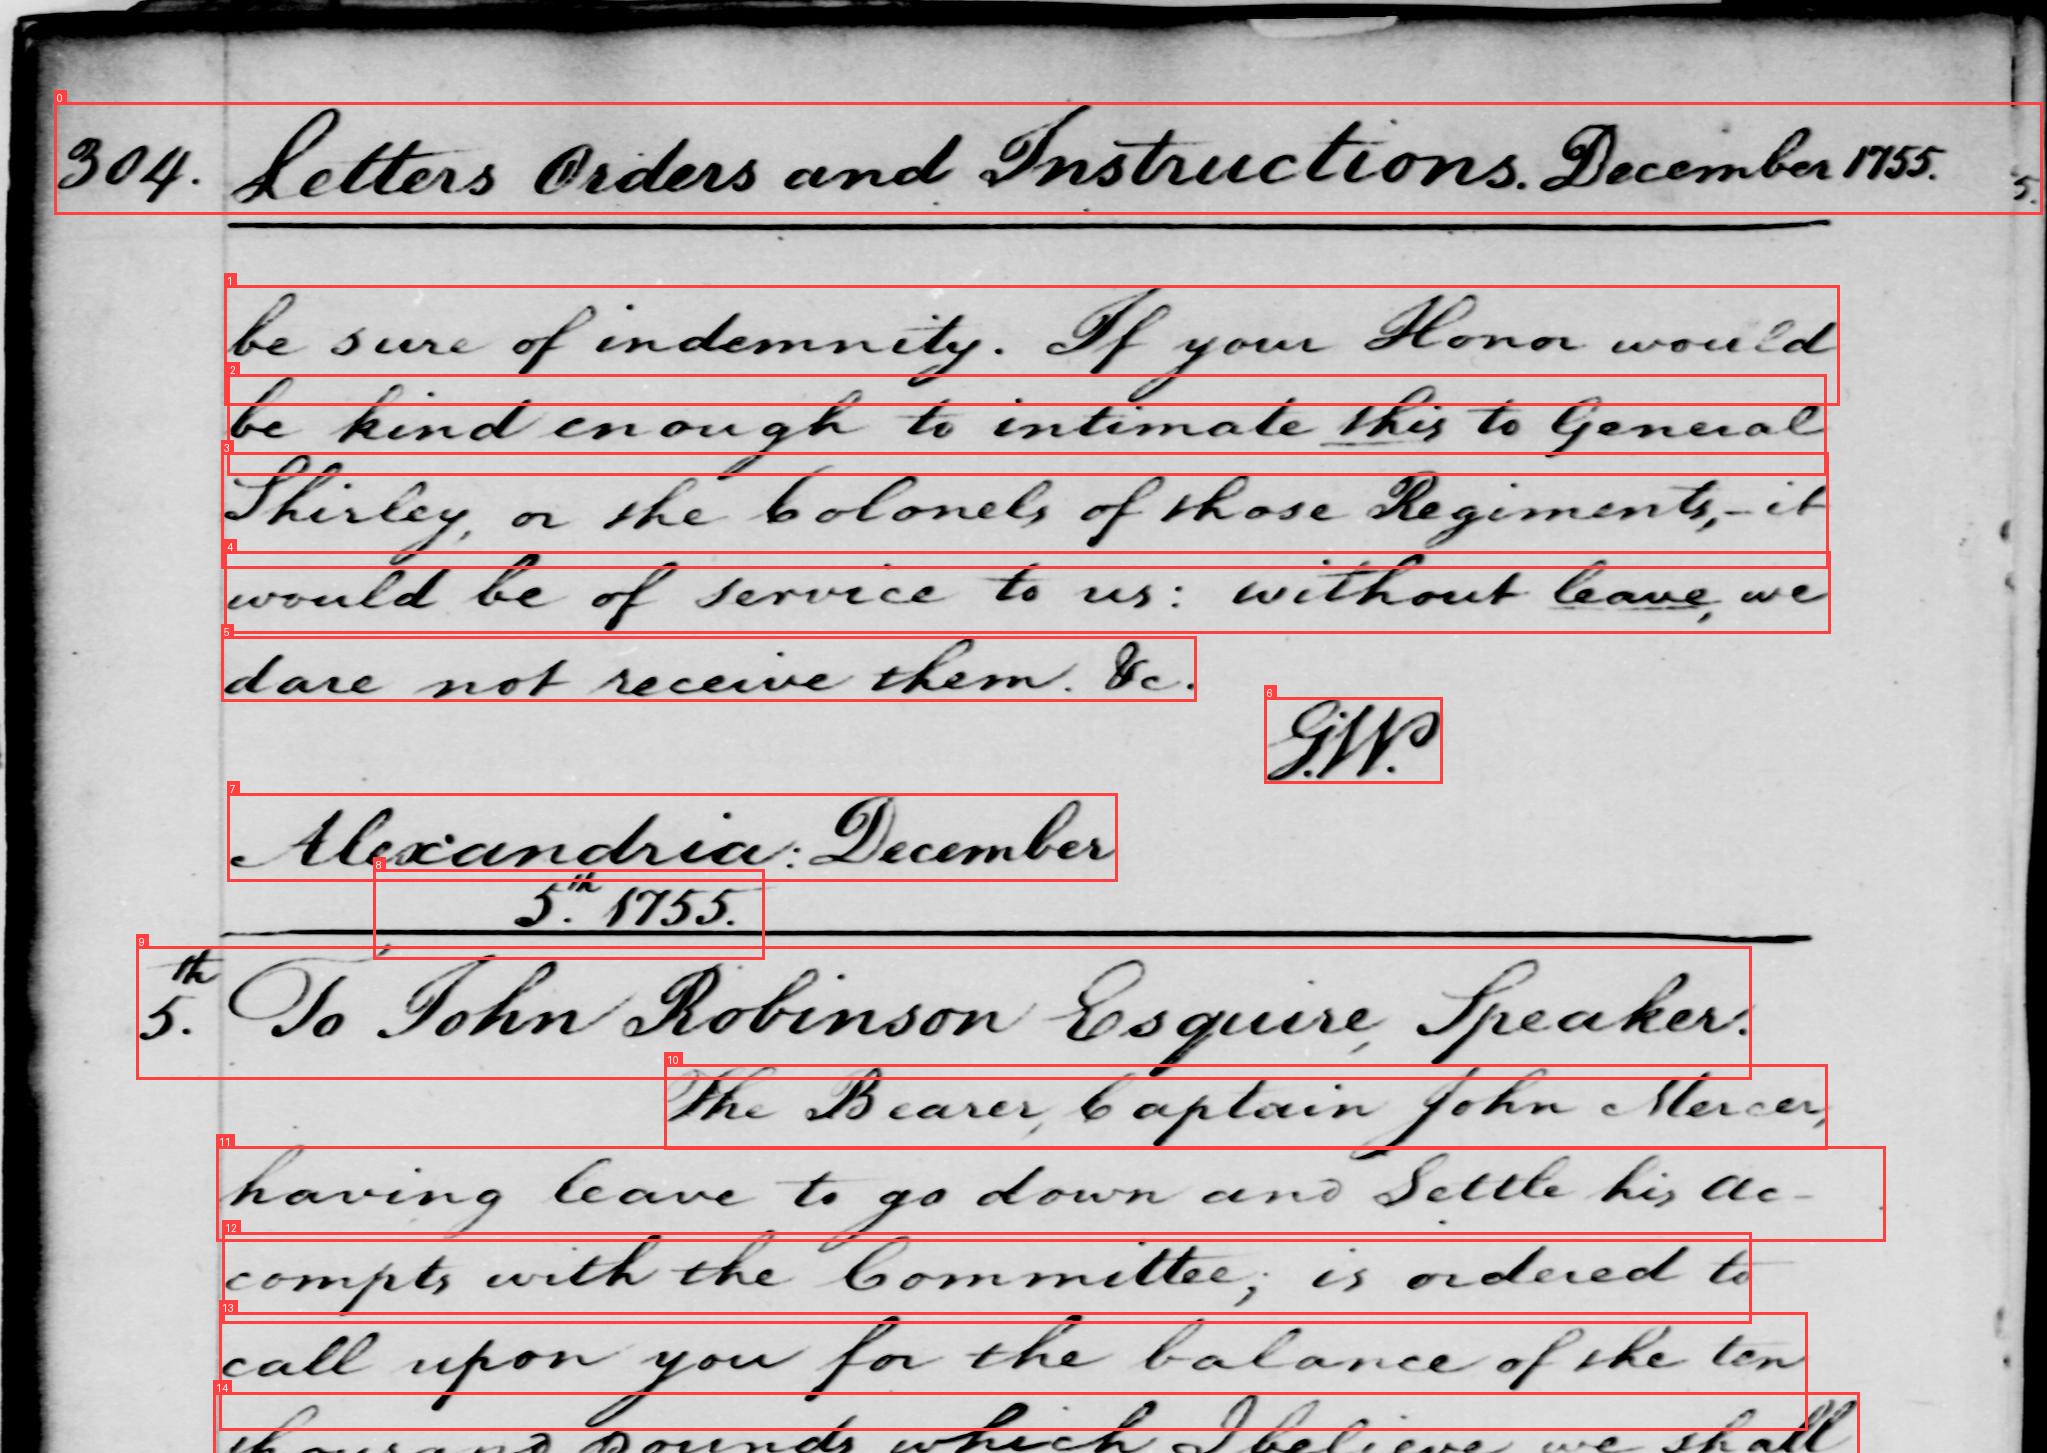
\includegraphics[width=0.92\linewidth]{images/pdf_optimized/ch6_washington_304_overlay_crop.jpg}
  \caption{Cropped upper-region view of Washington sample 304 with OCR-line overlay. The crop shows the opening line scaffold discussed in the first row of Table~\ref{tab:exp_linebreak_comparison}, the full excerpt in Appendix Table~\ref{tab:app_qualitative_excerpt_blocks}, and the first qualitative paragraph. The example illustrates that the opening-line partition remains structurally relevant even when the selected M3 row already preserves the character content.}
  \label{fig:exp_qualitative_input_washington}
\end{figure}

\needlines{8}
\paragraph{Illustrative OCR-noise recovery.}
OCR-noise recovery gives a complementary mechanism. Children sample \texttt{3B\_19\_2-3}, shown as a cropped detail in Figure~\ref{fig:exp_qualitative_input_children} and excerpted in Appendix Table~\ref{tab:app_qualitative_ocr_excerpt}, is included as an \emph{illustrative} OCR-noise example rather than as a typical Children sample. Here M2 reaches \(\LANormCombinedToken=\LineFOneNormToken=0.286\) with \(\CERNormToken=0.190\), M3 improves to \(0.714\) on both line metrics with \(\CERNormToken=0.164\), and M5 reaches \(\LANormCombinedToken=\LineFOneNormToken=1.000\) with \(\CERNormToken=0.000\). The progression matters: The case is not purely ``M2 fails, M5 succeeds,'' because M3 already recovers much of the structure from OCR text alone. What makes the sample useful is that the remaining difference is consistent with a small local handwritten detail around the \texttt{\&} token that is easy to lose in OCR text but visible in local image evidence.

\begin{figure}[p]
  \centering
  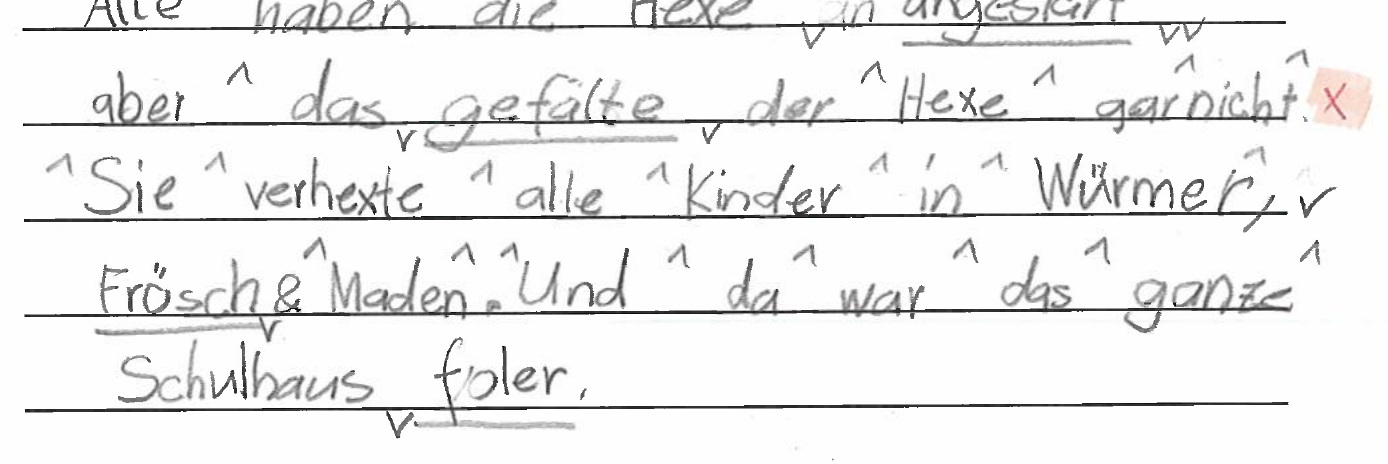
\includegraphics[width=0.90\linewidth]{images/pdf_optimized/ch6_children_3B_19_2-3_crop.jpg}
  \caption{Selected Children Handwritten sample detail cropped for readability. The example illustrates OCR-noise recovery discussed in the second qualitative paragraph: The local handwritten detail around the \texttt{\&} token is visible in the image and is consistent with the additional structure recovery in the reported M5 setup beyond OCR-conditioned text alone.}
  \label{fig:exp_qualitative_input_children}
\end{figure}

\paragraph{Why IAM is already easy for OCR-grounded methods.}
IAM shows the absence of measurable headroom. Sample \texttt{p06-042} is a plateau case rather than an M5-specific gain case: M3/\GPTFiveMarchShort{}, M4/\GPTFiveMarchShort{}, M5/\GPTFiveShort{}, and NNTP/NNTP all reach \(\LANormCombinedToken=\LineFOneNormToken=1.000\) with \(\CERNormToken=0.000\). That is precisely why it belongs in the qualitative analysis. It shows that some cleaner modern handwritten subsets are already almost solved once OCR line order is close to the ground truth, so richer image evidence does not necessarily create a new advantage; instead, it confirms a structure that is already largely recoverable from OCR-conditioned inputs.

\paragraph{Bullinger high-F1 positional failure.}
Bullinger supplies the sharpest positional rather than lexical failure. Sample 12517, summarized in the third row of Table~\ref{tab:exp_linebreak_comparison} and excerpted in Appendix Table~\ref{tab:app_qualitative_excerpt_blocks}, is the clearest high-\LineFOneNorm{} / low-\LANormCombined{} case already used in the qualitative table. The selected M1/\GPTFiveMarchShort{} row drops the opening line \texttt{234}, which is enough to force \(\LANormCombinedToken=0.000\) even though \(\LineFOneNormToken=0.909\), with \(\CERNormToken=0.006\). The matched M5/\GPTFiveShort{} row reaches \(\LANormCombinedToken=\LineFOneNormToken=1.000\) and \(\CERNormToken=0.000\). Many line strings survive as exact normalized strings, but the sequence-level alignment fails completely after the opening omission.

\paragraph{A boundary case for M5 interpretation.}
The final case bounds the M5 interpretation from the other direction by showing a page where an earlier LLM/VLM-based configuration is stronger. The fifth row of Table~\ref{tab:exp_linebreak_comparison}, expanded in Appendix Table~\ref{tab:app_qualitative_excerpt_blocks}, shows this directly for Washington sample 270: M3/\GPTFiveMarchShort{} reaches \(\LANormCombinedToken=\LineFOneNormToken=0.935\) with \(\CERNormToken=0.002\), while the selected M5/\QwenThirtyTwoShort{} row drops to \(0.871\) on both line metrics with the same \(\CERNormToken=0.002\). The M5 trace records \texttt{fallback\_projection} after \texttt{initial+repair}; the stored prediction locally over-splits the hyphenated \texttt{Recrui-\textbackslash nting} boundary as \texttt{Recrui\textbackslash n- ting}. The same sample is also the clearest NNTP-favored case against the matched Washington M5 row: The Washington NNTP fold prediction preserves the ground-truth split and reaches \(\LANormCombinedToken=\LineFOneNormToken=1.000\) with \(\CERNormToken=0.000\). Including this boundary case keeps the qualitative analysis aligned with the aggregate result: It illustrates trace and error patterns without turning an individual sample into the full RQ3 answer.

\FloatBarrier

\section{Interpretation and Validity Boundaries}
\label{sec:experimentation_analysis}

\paragraph{Supported interpretation.}
The clearest empirical pattern comes from reading the main handwritten overview together with the controlled LLM/VLM-based checks. M5 has the highest reported macro score among the evaluated LLM/VLM-based alignment setups in the overview table, and it remains highest wherever the exact-model comparison is complete. At the same time, the intermediate steps are not monotonic: M3 can already perform strongly on cleaner or OCR-friendly material, and M4 does not uniformly improve over M3. The supported conclusion is therefore about the reported evidence-and-control mix, with M5 interpreted as the evaluated context-rich line-image setup rather than as a universal stepwise ladder from M1 to M5.

\paragraph{Validity-boundary synthesis.}
The main boundaries are consolidated in Table~\ref{tab:exp_validity_boundaries}. They define the level at which the result tables should be read and preserve the chapter's main result: The reported evidence is most secure at the level of evaluated alignment setups, not isolated components.

\begin{table}[!htbp]
  \centering
  \caption{Compact interpretation boundaries for the Chapter~\ref{cha:experimentation} result layers. The table summarizes how dataset staging, provider provenance, output control, NNTP preprocessing, and sample-set availability bound the reported comparisons.}
  \label{tab:exp_validity_boundaries}
  \scriptsize
  \renewcommand{\arraystretch}{1.12}
  \setlength{\tabcolsep}{2.5pt}
  \begin{tabularx}{\linewidth}{@{}>{\raggedright\arraybackslash}p{0.20\linewidth}>{\raggedright\arraybackslash}p{0.31\linewidth}X@{}}
    \toprule
    \textbf{Boundary} & \textbf{Affects} & \textbf{Consequence for interpretation} \\
    \midrule
    Known-count staging for M4/M5 & Structured rows in Tables~\ref{tab:exp_handwritten_main_overview}, \ref{tab:exp_handwritten_controlled_model}, \ref{tab:exp_line_count_drift}, and \ref{tab:exp_method_weakness_mechanisms}; comparability summaries in Tables~\ref{tab:method_comparability_matrix} and \ref{tab:app_method_comparability_matrix_full}. & M4 and M5 test boundary assignment under known-count staging: The handwritten \texttt{ocr\_lines} cardinality matches the ground-truth line count. They are not blind page-side line-count or segmentation systems. \\
    \addlinespace[0.35em]
    Mixed line-crop provenance & M5 and NNTP rows in Tables~\ref{tab:exp_handwritten_main_overview}, \ref{tab:exp_best_vs_nntp}, \ref{tab:exp_bullinger_contextual}, and \ref{tab:exp_linebreak_comparison}. & Children Handwritten and IAM use dataset-provided line images, Bullinger uses PAGE/XML-derived crops, and Washington uses curated Kraken crops. The comparison is among evaluated configurations with their respective anchors, not among crop-generation pipelines. \\
    \addlinespace[0.35em]
    Model-configuration dependence & Overview and provenance tables: Tables~\ref{tab:exp_handwritten_main_overview}, \ref{tab:exp_handwritten_prompt_matrix}, \ref{tab:app_handwritten_prompt_provenance}, and \ref{tab:app_handwritten_prompt_detail_metrics}; controlled checks in Tables~\ref{tab:exp_handwritten_controlled_model} and \ref{tab:app_mistral_fixed_provider_matrix}. & The overview may use different model configurations across cells. M5 remains the highest-scoring row in the reported overview and in the exact-model OpenAI control, while intermediate M1--M4 rankings remain model- and dataset-sensitive. \\
    \addlinespace[0.35em]
    Projection versus raw returned text & M1--M5 comparisons in Tables~\ref{tab:exp_handwritten_main_overview} and \ref{tab:exp_handwritten_controlled_model}; line-count drift in Table~\ref{tab:exp_line_count_drift}; M5 traces in Table~\ref{tab:app_m5_trace_event_counts}; mechanisms in Table~\ref{tab:exp_method_weakness_mechanisms}. & M1--M3 score raw returned text, whereas M4/M5 may validate, repair, recover, fall back, and project a boundary plan onto the supplied transcription. This improves fixed-transcription validity but does not isolate projection, repair, fallback, or JSON validity as separate causes. \\
    \addlinespace[0.35em]
    Heuristic multi-page chunking for M1/M2 & Raw page-image regimes in Tables~\ref{tab:exp_handwritten_main_overview}, \ref{tab:exp_handwritten_controlled_model}, and \ref{tab:exp_method_weakness_mechanisms}. & The affected handwritten samples are multi-page Bullinger cases: 31/162 overall and 31/59 within Bullinger. M1/M2 results are evidence about the implemented chunked configurations, not isolated page-image or OCR/HTR hint effects. \\
    \addlinespace[0.35em]
    NNTP symbol-inventory preprocessing & NNTP rows in Tables~\ref{tab:exp_best_vs_nntp}, \ref{tab:exp_bullinger_contextual}, and \ref{tab:exp_linebreak_comparison}; audit summary in Table~\ref{tab:app_nntp_symbol_filter_audit}. & NNTP applies symbol-inventory preprocessing before alignment. The shared line-metric comparison remains useful; character-level comparisons against M1--M5 need this preprocessing caveat. \\
    \addlinespace[0.35em]
    Sample-set mismatch and small samples & NNTP comparison tables, especially Tables~\ref{tab:exp_best_vs_nntp} and \ref{tab:exp_bullinger_contextual}; cross-dataset readings of Tables~\ref{tab:exp_handwritten_main_overview} and \ref{tab:exp_handwritten_controlled_model}. & Children and Washington use NNTP cross-validation macro summaries, IAM uses a legacy single run, Bullinger lacks a thesis-side matched full-sample NNTP row, and IAM/Washington each have \(n=20\). The M5--NNTP result is close and dataset-dependent rather than one homogeneous winner. \\
    \addlinespace[0.35em]
    Missing deterministic scaffold baselines & Causal readings of Tables~\ref{tab:exp_handwritten_main_overview}, \ref{tab:exp_handwritten_controlled_model}, \ref{tab:exp_line_count_drift}, \ref{tab:app_m5_trace_event_counts}, and \ref{tab:exp_method_weakness_mechanisms}. & The result set does not include full-sample deterministic controls such as OCR-line dynamic alignment, known-\(N\) proportional splitting, OCR-only projection, or no-projection M4/M5 ablations. The observed gains belong to reported configurations rather than to isolated scaffold components. \\
    \bottomrule
  \end{tabularx}
\end{table}

\FloatBarrier

\paragraph{Chapter summary.}
\label{sec:experimentation_summary}

Taken together, the experiments support a comparison of reported alignment setups with different evidence and output control rather than isolated components. M5 has the highest reported macro score among the evaluated LLM/VLM-based handwritten alignment setups, and the controlled checks preserve this main result wherever complete comparisons exist. The printed rows add limited M1--M3 modality context, while the NNTP comparison shows that deterministic forced alignment remains a competitive reference point. The result is therefore an evidence base for newline-only transcription alignment under increasingly structured evidence and output control, with the main interpretation boundaries summarized in Table~\ref{tab:exp_validity_boundaries}.
